\subsubsection{Use Cases (including text narratives)}
The following use case diagram makes the assumption that all data stored 
on the blockchain is valid and authentic. The external blockchain system will 
be treated as an actor in the text narratives below.

\begin{figure}[h]
\centering % centre is you want
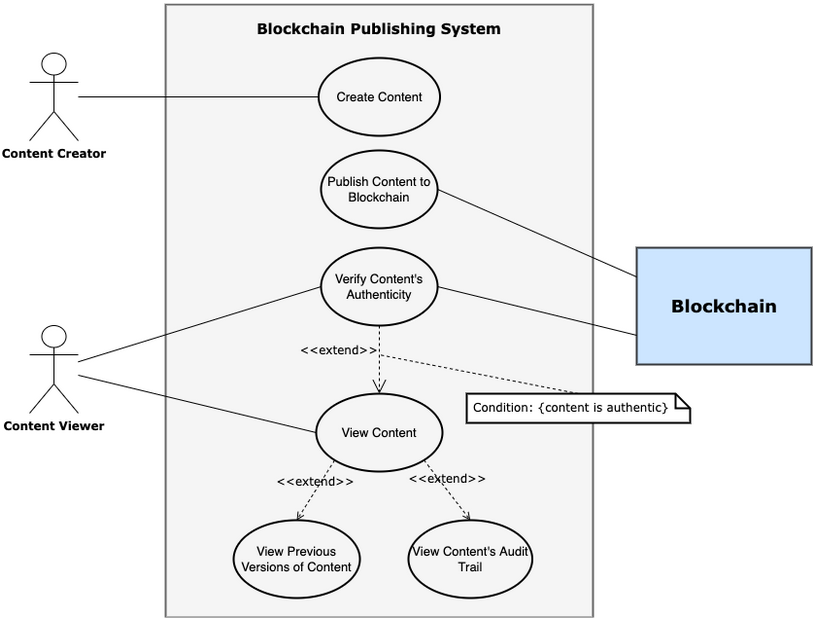
\includegraphics[scale=0.50]{use-case-content} % To learn more go to: https://www.overleaf.com/learn/latex/Inserting_Images 
\caption{Use case diagram of the system}
\label{fig: create-content} % Can be used with function \ref{fig: passion-fruit-flower} to reference to image
\end{figure}

\noindent
\textbf{Textual Description of “Create Content”:} \\
\textit{Actors involved:} Content Creator \\ \\
\textit{Precondition:} An individual or organisation wishes to create a piece of content 
					   (e.g a blog post) to be published by the system. \\ \\
\textit{Normal Scenario:} The content creator creates a piece of content and submits it to the system. \\ \\
\textit{Post Condition:} The content is published to the blockchain. \\ \\
\textit{Error Scenario:} The system crashes and the content is lost and not passed into the system. \\ \\

\noindent
\textbf{Textual Description of “Publish Content to Blockchain”:} \\
\textit{Actors involved:} Blockchain  \\ \\
\textit{Precondition:} 
	\begin{itemize}
		\item The content creator has submitted some form of content to the system to be published.
		\item The system has access to the blockchain network. 
	\end{itemize}
\textit{Normal Scenario:} A new block which includes the content data, metadata, and previous hash of the block
						  these are all added to the blockchain. \\ \\
\textit{Special Scenario:} If there are no prexisting blocks, the block created will be a Genesis block,
						   this block does not store a hash of the previous block, as there is no previous block. \\ \\
\textit{Post Condition:} The content is now stored on the blockchain and can be accessed by the system 
						 and published for user’s to view. \\ \\
\textit{Error Scenario:} The new block cannot be added to the blockchain due to lack of funds 
						 or error within the system. \\ \\

\noindent
\textbf{Textual Description of “Verify Content's Authenticity”:} \\
\textit{Actors involved:} Content Viewer, Blockchain \\ \\
\textit{Precondition:} 
	\begin{itemize}
		\item Content has been published to the blockchain.
		\item The block containing the content on the blockchain has not been tampered with.
	\end{itemize}
\textit{Normal Scenario:} The system has reference to the block on the blockchain which 
						  contains the content the user wishes to view. \\ \\
\textit{Post Condition:} The verified content can be viewed by the user through the web application. \\ \\
\textit{Error Scenario:} The block has been tampered with and the content can no longer be deemed valid or authentic. \\ \\

\newpage
\noindent
\textbf{Textual Description of “View Content”:} \\
\textit{Actors involved:} Content Viewer \\ \\
\textit{Precondition:} 
	\begin{itemize}
		\item The content viewer has selected a piece of content they wish to view.
		\item The content has been authenticated by the system. 
	\end{itemize}
\textit{Normal Scenario:} The user accesses the web application and chooses a piece of content 
					      they wish to view. That content is then displayed to the user. \\ \\
\textit{Post Condition:} The user has access to verified content and can view previous versions 
						 of the content as well as the content’s audit trail. \\ \\
\textit{Error Scenario:} The content is wrongly deemed valid due to a system error and 
						 the tampered content is presented to the user. \\ \\

\noindent
\textbf{Textual Description of “View Previous Versions of Content”:} \\
\textit{Actors involved:} Content Viewer \\ \\	
\textit{Precondition:} 
	\begin{itemize}
		\item System error causes previous versions of the content to be lost and inaccessible to the user. 
		\item Each of these versions has been verified.
	\end{itemize}
\textit{Normal Scenario:} The user can switch between different versions of the piece of content 
						  they are viewing and see the differences between each version, 
						  as well as who made the changes. \\ \\
\textit{Post Condition:} The user has an overview of how the content came to be and by whom. \\ \\
\textit{Error Scenario:} System error causes previous versions of the content to be lost and inaccessible to the user.\\ \\

\newpage
\noindent
\textbf{Textual Description of “View Content's Audit Trail”:} \\
\textit{Actors involved:} Content Viewer \\ \\
\textit{Precondition:} 
	\begin{itemize}
		\item There is at least one version of the content published to the system.
		\item The changes made, as well as when the changes were made and by whom are stored in the blockchain.
	\end{itemize}
\textit{Normal Scenario:} The user can see a list of the various versions of the 
						  piece of content as well as the type of change made 
						  (e.g creation, edit), the date, and the author. \\ \\
\textit{Post Condition:} The user can access the various versions of the content through 
						 the clicking on the relevant version on the audit log as well as 
						 get an overview of how the content came to be. \\ \\
\textit{Error Scenario:} Changes to the content are lost or unverifiable due to system error 
						 and the information shown in the audit log is inaccurate. \\ \\
\newpage
